\documentclass{scrartcl}
\usepackage{physics}   % Matrices and Dirac-notation
\usepackage{amsmath}   % Binear equations
\usepackage{booktabs}  % Tabs
\usepackage{graphicx}  % Pictures/figures
\usepackage{listings}  % Source code
\usepackage{color}     % Colors
\usepackage{mdframed}  % Frames
\usepackage{float}

\definecolor{dkgreen}{rgb}{0,0.6,0}
\definecolor{gray}{rgb}{0.5,0.5,0.5}
\definecolor{mauve}{rgb}{0.58,0,0.82}

%Defining source code
\lstset{frame=tb,
  language=Python,
  aboveskip=3mm,
  belowskip=3mm,
  showstringspaces=false,
  columns=flexible,
  basicstyle={\small\ttfamily},
  numbers=none,
  numberstyle=\tiny\color{gray},
  keywordstyle=\color{blue},
  commentstyle=\color{dkgreen},
  stringstyle=\color{mauve},
  breaklines=true,
  breakatwhitespace=true,
  tabsize=3
}
\makeatletter
\renewcommand*\env@matrix[1][*\c@MaxMatrixCols c]{%
  \hskip -\arraycolsep
  \let\@ifnextchar\new@ifnextchar
  \array{#1}}
\makeatother
\begin{document}
\begin{titlepage}
	\centering
	
\includegraphics[width=0.15\textwidth]{uio.png}\par\vspace{1cm}
	{\scshape\LARGE FYS3110 - Quantum Mechanics \par}
	\vspace{1cm}
	{\scshape\Large University of Oslo\par}
	\vspace{5.5cm}
	{\huge\bfseries Home Exam 2016\par}
	\vspace{1.5cm}
	{\Large\itshape Candidate number: 54\par}
	\vfill
	{\large October 15, 2016\par}
\end{titlepage}

\section*{Problem 1}
In this project we are studying different spin-1/2 systems, first with one spin-1/2, and thereafter a system with three spin-1/2. Below I will list all the relations given, so I can refer to them later in the problem. \par\vspace{2mm}
First we are given the general relation
\begin{equation}
\hat{S}^2=\hat{S}_x^2+\hat{S}_y^2+\hat{S}_z^2
\label{eq:S2}
\end{equation}
We define the states $\ket{S=1/2,m_s=\pm1/2}$ as
\begin{equation}
\ket{\uparrow}\equiv\ket{S=1/2,m_s=+1/2}
\end{equation}
\begin{equation}
\ket{\downarrow}\equiv\ket{S=1/2,m_s=-1/2}
\end{equation}
to shorten down the notation. Those are eigenstates of $\hat{S}^2$ and $\hat{S}_z$:
\begin{equation}
S^2\ket{\uparrow}=\hbar^2\frac{1}{2}\bigg(\frac{1}{2}+1\bigg)\ket{\uparrow}
\label{eq:S2up}
\end{equation}
\begin{equation}
S^2\ket{\downarrow}=\hbar^2\frac{1}{2}\bigg(\frac{1}{2}+1\bigg)\ket{\downarrow}
\label{eq:S2down}
\end{equation}
\begin{equation}
\hat{S}_z\ket{\uparrow}=+\frac{\hbar}{2}\ket{\uparrow}
\label{eq:Szup}
\end{equation}
\begin{equation}
\hat{S}_z\ket{\downarrow}=-\frac{\hbar}{2}\ket{\downarrow}
\label{eq:Szdown}
\end{equation}
We are also given the commutators between $\hat{S}_x$, $\hat{S}_y$ and $\hat{S}_z$:
\begin{equation}
[\hat{S}_x,\hat{S}_y]=i\hbar\hat{S}_z
\label{eq:Sxcom}
\end{equation}
\begin{equation}
[\hat{S}_y,\hat{S}_z]=i\hbar\hat{S}_x
\label{eq:Sycom}
\end{equation}
\begin{equation}
[\hat{S}_z,\hat{S}_x]=i\hbar\hat{S}_y
\label{eq:Szcom}
\end{equation}
The last relation given is
\begin{equation}
\hat{S}_\pm=\hat{S}_x\pm\hat{S}_y
\label{eq:Spm}
\end{equation}
Which easily can be transformed into
\begin{equation}
\hat{S}_x=\frac{1}{2}\bigg(\hat{S}_++\hat{S}_-\bigg)
\label{eq:Sx}
\end{equation}
\begin{equation}
\hat{S}_y=\frac{1}{2i}\bigg(\hat{S}_+-\hat{S}_-\bigg)
\label{eq:Sy}
\end{equation}
by calculating $\hat{S}_+\pm\hat{S}_-$. 

\subsection*{1.1}
A state is an eigenstate of an operator if the state is conserved while it is used on the operator. More concrete, we will in this exercise expect to get a result like $\hat{S}_z\hat{S}_+\ket{\downarrow}=c\hat{S}_+\ket{\downarrow}$ if $\hat{S_+}\ket{\downarrow}$ is an eigenstate of $\hat{S}_z$, where $c$ is the eigenvalue.
\begin{equation*}
\hat{S}_z\hat{S}_+\ket{\downarrow}=\hat{S}_z(\hat{S}_x+i\hat{S}_y)\ket{\downarrow}=(\hat{S}_z\hat{S}_x+ i\hat{S}_z\hat{S}_y)\ket{\downarrow}
\end{equation*}
Furthermore I will use the general relations $\hat{S}_z\hat{S}_x=[\hat{S}_z,\hat{S}_x]+\hat{S}_x\hat{S}_z$ and $\hat{S}_z\hat{S}_y=[\hat{S}_z,\hat{S}_y]+\hat{S}_y\hat{S}_z$, and the commutation relations given in Equation (\ref{eq:Sxcom}) and (\ref{eq:Sycom}). Remember $[\hat{A},\hat{B}]=-[\hat{B},\hat{A}]$!
\begin{equation*}
\Rightarrow \hat{S}_z\hat{S}_+\ket{\downarrow}=-i\hbar\hat{S}_y\ket{\downarrow}+\hat{S}_x\hat{S}_z\ket{\downarrow}-i^2\hbar\hat{S}_x\ket{\downarrow}+i\hat{S}_y\hat{S}_z\ket{\downarrow}
\end{equation*}
$\hat{S}_z\ket{\downarrow}$ pops up two times, but we can "kill" it using Equation (\ref{eq:Szdown}).
\begin{equation*}
\Rightarrow \hat{S}_z\hat{S}_+\ket{\downarrow}=-i\hbar\bigg(\frac{3}{2}\hat{S}_y+\frac{i}{2}\hat{S}_x\bigg)\ket{\downarrow}=\frac{\hbar}{2}(\hat{S}_x-i\hat{S}_y-2i\hat{S}_y)\ket{\downarrow}
\end{equation*}
The first two terms are equal to $\hat{S}_-$ (see Equation (\ref{eq:Spm})), while the last one is equal to $\hat{S}_--\hat{S}_+$ (Equation (\ref{eq:Sy})). The result is
\begin{equation}
\hat{S}_z\hat{S}_+\ket{\downarrow}=\underline{-\frac{\hbar}{2}\hat{S}_+\ket{\downarrow}}
\end{equation}
So $\hat{S}_+\ket{\downarrow}$ is an eigenfunction of $\hat{S}_z$ with eigenvalue $-\hbar/2$.

\subsection*{1.2}
From here I will omit the operator hats to simplify the notation. 
$$S_-S_+=(S_x-iS_y)(S_x+iS_y)=S_x^2+iS_xS_y-iS_yS_x+S_y^2=S_x^2+i[S_x,S_y]+S_y^2$$
Here I have to use Equation (\ref{eq:S2}) and (\ref{eq:Sxcom}), and we obtain 
\begin{equation*}
\Rightarrow S_-S_+=S^2-S_z^2-\hbar S_z
\label{eq:S-S+}
\end{equation*}
$$\braket{\psi_1}{\psi_1}=\mel{\downarrow}{S_-S_+}{\downarrow}=\mel{\downarrow}{S^2-S_z^2-\hbar S_z}{\downarrow}=\bra{\downarrow}(S^2\ket{\downarrow}-S_z^2\ket{\downarrow}-\hbar S_z\ket{\downarrow})$$
$$\braket{\psi_2}{\psi_2}=\mel{\uparrow}{S_-S_+}{\uparrow}=\mel{\uparrow}{S^2-S_z^2-\hbar S_z}{\uparrow}=\bra{\uparrow}(S^2\ket{\uparrow}-S_z^2\ket{\uparrow}-\hbar S_z\ket{\uparrow})$$
We can do this since $S_+$ and $S_-$ are hermitian conjugate of each other. Again I need the expressions from the description, and by combining Equation (\ref{eq:S2up}), (\ref{eq:S2down}), (\ref{eq:Szup}) and (\ref{eq:Szdown}), and using the fact that the inner product between two similar spin states are equal to 1, we get
\begin{equation}
\braket{\psi_1}{\psi_1}=\mel{\downarrow}{\bigg(\frac{3\hbar^2}{4}-\frac{\hbar^2}{4}+\frac{\hbar^2}{2}\bigg)}{\downarrow}=\bigg(\frac{3\hbar^2}{4}-\frac{\hbar^2}{4}+\frac{\hbar^2}{2}\bigg)\braket{\downarrow}{\downarrow}=\underline{\hbar^2}
\end{equation}
\begin{equation}
\braket{\psi_2}{\psi_2}=\mel{\uparrow}{\bigg(\frac{3\hbar^2}{4}-\frac{\hbar^2}{4}-\frac{\hbar^2}{2}\bigg)}{\uparrow}=\bigg(\frac{3\hbar^2}{4}-\frac{\hbar^2}{4}-\frac{\hbar^2}{2}\bigg)\braket{\uparrow}{\uparrow}=\underline{0}
\end{equation}\par\vspace{1cm}

I still have not mentioned what the $\hat{S}_\pm$ operators are. They are the spin ladder operators, where $\hat{S}_+$ has the property raising the secondary spin quantum number ($m_s$) and $\hat{S}_-$ does the opposite. In our case, we have two possible values for $m_s$: $+1/2$ and $-1/2$. This results in the given relations:
\begin{equation}
\hat{S}_+\ket{\downarrow}=\hbar\ket{\uparrow}
\label{eq:S+down}
\end{equation}
\begin{equation}
\hat{S}_-\ket{\uparrow}=\hbar\ket{\downarrow}
\label{eq:S-up}
\end{equation}
But we can also write down the two remaining combinations, since we know that the secondary spin quantum number only can be $+1/2$ and $-1/2$:
\begin{equation}
\hat{S}_+\ket{\uparrow}=0
\label{eq:S+up}
\end{equation}
\begin{equation}
\hat{S}_-\ket{\downarrow}=0
\label{eq:S-down}
\end{equation}

\subsection*{1.3}
In this exercise I will compute the variance of $S_x$ and $S_y$ ($\sigma_{S_x}^2$ and $\sigma_{S_y}^2$) where we are given a ket 
\begin{equation}
\ket{\phi}=\frac{1}{\sqrt{2}}(\ket{\uparrow}+e^{i\theta}\ket{\downarrow}).
\end{equation}
The corresponding bra is given by
\begin{equation*}
\bra{\phi}=(\ket{\phi})^\dagger=\frac{1}{\sqrt{2}}(\bra{\uparrow}+e^{-i\theta}\bra{\downarrow})
\end{equation*}
After done these calculations, we will compute the "uncertainly" product and compare it with the solution of the general uncertainly relation. The "uncertainly" product is given by 
\begin{equation*}
\sigma_{S_x}^2\sigma_{S_y}^2=\mel{\phi}{(S_x-\mel{\phi}{S_x}{\phi})^2}{\phi}\mel{\phi}{(S_y-\mel{\phi}{S_y}{\phi})^2}{\phi}
\end{equation*}
This will be really out of hand if we compute it directly, so let's split it up!
\begin{equation*}
\mel{\phi}{(S_x-\mel{\phi}{S_x}{\phi})^2}{\phi}=\mel{\phi}{(S_x^2-2S_x\mel{\phi}{S_x}{\phi}+\mel{\phi}{S_x}{\phi}^2)}{\phi}
\end{equation*}
\begin{equation*}
=\mel{\phi}{S_x^2}{\phi}-2\mel{\phi}{S_x\mel{\phi}{S_x}{\phi}}{\phi}+\mel{\phi}{\mel{\phi}{S_x}{\phi}^2}{\phi}
\end{equation*}
\begin{equation*}
=\mel{\phi}{S_x^2}{\phi}-2\mel{\phi}{S_x}{\phi}\mel{\phi}{S_x}{\phi}+\mel{\phi}{S_x}{\phi}^2\braket{\phi}{\phi}
\end{equation*}
\begin{equation*}
=\mel{\phi}{S_x^2}{\phi}-\mel{\phi}{S_x}{\phi}^2
\end{equation*}
Where I have used that the expectation value is a constant and that the inner product between two similar states is equal to one (the states are normalized). So we just have to calculate two expectation values. I will need Equation (\ref{eq:Sx}), (\ref{eq:Sy}), (\ref{eq:S+down}), (\ref{eq:S-up}), (\ref{eq:S+up}) and (\ref{eq:S-down}).
\begin{equation*}
\mel{\phi}{S_x}{\phi}=\bra{\phi}\frac{1}{2}(S_++S_-)\cdot \frac{1}{\sqrt{2}}(\ket{\uparrow}+e^{i\theta}\ket{\downarrow})
\end{equation*}
\begin{equation*}
=\bra{\phi}\frac{1}{2\sqrt{2}}(S_+\ket{\uparrow}+S_-\ket{\uparrow}+e^{i\theta}S_+\ket{\downarrow}+e^{i\theta}S_-\ket{\downarrow})
\end{equation*}
\begin{equation*}
=\frac{\hbar}{4}(\bra{\uparrow}+e^{-i\theta}\bra{\downarrow})(\ket{\downarrow}+e^{i\theta}\ket{\uparrow})
\end{equation*}
\begin{equation*}
=\frac{\hbar}{4}(\braket{\uparrow}{\uparrow}+e^{i\theta}\braket{\uparrow}{\downarrow}+e^{-i\theta}\braket{\downarrow}{\downarrow}+e^0\braket{\downarrow}{\uparrow})=\frac{\hbar}{4}(e^{i\theta}+e^{-i\theta})
\end{equation*}
By combining Euler's formula, we can find the relation $e^{i\theta}+e^{-i\theta}=2\cos\theta$, and finally we obtain
\begin{equation}
\mel{\phi}{S_x}{\phi}=\underline{\frac{\hbar}{2}\cos\theta}
\end{equation}
We also need $\mel{\phi}{S_x^2}{\phi}$:
\begin{equation*}
S_x^2\ket{\phi}=\frac{1}{4}(S_+^2+S_+S_-+S_-S_++S_-^2)\ket{\phi}
\end{equation*}
\begin{equation*}
=\frac{1}{4\sqrt{2}}(S_+^2\ket{\uparrow}+S_+S_-e^{i\theta}\ket{\downarrow}+S_-S_+\ket{\uparrow}+S_-^2e^{i\theta}\ket{\downarrow}+S_+^2\ket{\uparrow}+S_+S_-e^{i\theta}\ket{\downarrow}+S_-S_+\ket{\uparrow}+S_-^2e^{i\theta}\ket{\downarrow})
\end{equation*}
From Equation (\ref{eq:S+up}) and (\ref{eq:S-down}) we can see that all terms where we get $S_+\ket{\uparrow}$ or $S_-\ket{\downarrow}$ need to be equal to zero, so we obtain
\begin{equation*}
S_x^2\ket{\phi}=\frac{\hbar^2}{4\sqrt{2}}(\ket{\uparrow}+e^{i\theta}\ket{\downarrow})=\frac{\hbar^2}{4}\ket{\phi}
\end{equation*}
So $\ket{\phi}$ is an eigenket of $S_x^2$ with eigenvalue $\frac{\hbar^2}{4}$!
\begin{equation}
\mel{\phi}{S_x^2}{\phi}=\frac{\hbar^2}{4}\braket{\phi}{\phi}=\underline{\frac{\hbar^2}{4}}
\end{equation}
Since $\ket{\phi}$ is already normalized:
\begin{equation*}
\braket{\phi}{\phi}=\frac{1}{\sqrt{2}}(\bra{\downarrow}+e^{-i\theta}\bra{\uparrow}) \frac{1}{\sqrt{2}}(\ket{\downarrow}+e^{i\theta}\ket{\uparrow})=\frac{1}{2}(1+0+0+1)=1
\end{equation*}

Finally we obtain 
\begin{equation}
\mel{\phi}{(S_x-\mel{\phi}{S_x}{\phi})^2}{\phi}=\mel{\phi}{S_x^2}{\phi}-\mel{\phi}{S_x}{\phi}^2=\frac{\hbar^2}{4}-\bigg(\frac{\hbar}{2}\cos\theta\bigg)^2
\end{equation}

The next step is to do all this once again, but with $S_y$:
\begin{equation*}
\mel{\phi}{S_y}{\phi}=\bra{\phi}\frac{1}{2i}(S_+-S_-)\cdot \frac{1}{\sqrt{2}}(\ket{\uparrow}+e^{i\theta}\ket{\downarrow})
\end{equation*}
\begin{equation*}
=\bra{\phi}\frac{1}{2\sqrt{2}i}(S_+\ket{\uparrow}+S_-\ket{\uparrow}+e^{i\theta}S_+\ket{\downarrow}+e^{i\theta}S_-\ket{\downarrow})
\end{equation*}
\begin{equation*}
=\frac{\hbar}{4i}(\bra{\uparrow}-e^{-i\theta}\bra{\downarrow})(\ket{\downarrow}+e^{i\theta}\ket{\uparrow})
\end{equation*}
\begin{equation}
=\frac{\hbar}{4i}(e^{i\theta}\braket{\uparrow}{\uparrow}+\braket{\downarrow}{\uparrow}-\braket{\uparrow}{\downarrow}+e^{-i\theta}\braket{\downarrow}{\downarrow})=\frac{\hbar}{4i}(e^{i\theta}-e^{-i\theta})=\underline{\frac{\hbar}{2}\sin\theta}
\end{equation}
Where I again have used a result from Euler's formula: $e^{i\theta}-e^{-i\theta}=2i\sin\theta$.
We also need $\mel{\phi}{S_y^2}{\phi}$:
\begin{equation*}
S_y^2\ket{\phi}=-\frac{1}{4}(S_+^2-S_+S_--S_-S_++S_-^2)\frac{1}{\sqrt{2}}(\ket{\uparrow}+e^{i\theta}\ket{\downarrow})
\end{equation*}
\begin{equation*}
-\frac{1}{4\sqrt{2}}(-S_+S_-\ket{\uparrow}-e^{i\theta}S_-S_+\ket{\downarrow})=\frac{\hbar^2}{4}\ket{\phi}
\end{equation*}
$\ket{\phi}$ is an eigenstate of $S_y$ also, with the same eigenvalue as for $S_x$
\begin{equation}
\mel{\phi}{S_y^2}{\phi}=\underline{\frac{\hbar^2}{4}}
\end{equation}

We obtain 
\begin{equation}
\mel{\phi}{(S_y-\mel{\phi}{S_y}{\phi})^2}{\phi}=\mel{\phi}{S_y^2}{\phi}-\mel{\phi}{S_y}{\phi}^2=\frac{\hbar^2}{4}-\bigg(\frac{\hbar}{2}\sin\theta\bigg)^2
\end{equation}

The uncertainly relation is then
\begin{equation}
\sigma_{S_x}^2\sigma_{S_y}^2=\Bigg(\frac{\hbar^2}{4}-\bigg(\frac{\hbar}{2}\cos\theta\bigg)^2\Bigg)\Bigg(\frac{\hbar^2}{4}-\bigg(\frac{\hbar}{2}\sin\theta\bigg)^2\Bigg)=\bigg(\frac{\hbar^2}{4}\sin\theta\cos\theta\bigg)^2
\label{eq:sigma}
\end{equation}
So, is Heisenberg's uncertainty relation violated? The general uncertainty relation states 
\begin{equation*}
\sigma_A^2\sigma_B^2=(\langle[A,B]\rangle)^2
\end{equation*}
In our case, $A=S_x$ and $B=S_y$. By using Equation (\ref{eq:Sxcom}), we get
\begin{equation*}
\sigma_{S_x}^2\sigma_{S_y}^2=(\langle[S_x,S_y]\rangle)^2\geq\bigg(\frac{\hbar}{2}\langle S_z\rangle\bigg)^2=\frac{\hbar^2}{4}\langle S_z\rangle^2
\end{equation*}
We can find $\langle S_z\rangle^2$ with matrix representation:
\begin{equation*}
\langle S_z\rangle =\mel{\psi}{S_z}{\psi}
\end{equation*}
Where $\ket{\psi}$ is a eigenstate of $S_z$, which we represent by $\mqty(a\\b)$ and $S_z$ is represented by the matrix $\frac{\hbar}{2}\mqty(1&0\\0&-1)$
\begin{equation*}
\langle S_z\rangle=\frac{\hbar}{2}\mqty(a^*&b^*)\mqty(1&0\\0&-1)\mqty(a\\b)=\frac{\hbar}{2}\Big(|a|^2-|b|^2\Big)
\end{equation*}
$\ket{\phi}$ from above is obviously an eigenstate of $S_z$, with $a=\frac{1}{\sqrt{2}}$ and $b=\frac{e^{i\theta}}{\sqrt{2}}$.
\begin{equation*}
\langle S_z\rangle=\frac{\hbar}{2}\bigg(\frac{1}{2}-\frac{1}{2}\bigg)=0=\langle S_z\rangle^2
\end{equation*}
\begin{equation*}
\sigma_{S_x}^2\sigma_{S_y}^2\geq0
\end{equation*}
If we look at our expression for $\sigma_{S_x}^2\sigma_{S_y}^2$ in Equation (\ref{eq:sigma}), we can see that it will never be negative, and it follows therefore Heisenberg's uncertainly relation.

\subsection*{1.4}
In this exercise I will in the first place omit the tensor products
\begin{equation*}
\vec{S}_1\cdot\vec{S}_2=(S_1^x, S_1^y, S_1^z)\cdot(S_2^x, S_2^y, S_2^z)=S_1^xS_2^x+S_1^yS_2^y+S_1^zS_2^z
\end{equation*}
This is not a dot product! The lower index gives the position in the tensor product, for instance
\begin{equation*}
S_1^xS_2^x\equiv S^x\otimes S^x\otimes I
\end{equation*}
Where $I$ is the identity operator. Again we have to use Equation (\ref{eq:Sx}) and (\ref{eq:Sy}):
\begin{equation*}
\Rightarrow \frac{1}{4}(S_1^++S_1^-)(S_2^++S_2^-)-\frac{1}{4}(S_1^+-S_1^-)(S_2^+-S_2^-)+S_1^zS_2^z
\end{equation*}
\begin{equation*}
\frac{1}{4}(S_1^+S_2^++S_1^+S_2^-+S_1^-S_2^++S_1^-S_2^--S_1^+S_2^++S_1^+S_2^-+S_1^-S_2^+-S_1^-S_2^-)+S_1^zS_2^z
\end{equation*}
We can see that four of the terms cancel, and we have the expression
\begin{equation}
\vec{S}_1\cdot\vec{S}_2=\frac{1}{2}(S_1^+S_2^-+S_1^-S_2^+)+S_1^zS_2^z
\end{equation}
\begin{equation}
\vec{S}_2\cdot\vec{S}_3=\frac{1}{2}(S_2^+S_3^-+S_2^-S_3^+)+S_2^zS_3^z
\end{equation}
\begin{equation}
\vec{S}_3\cdot\vec{S}_1=\frac{1}{2}(S_3^+S_1^-+S_3^-S_1^+)+S_3^zS_1^z
\end{equation}
We can express the two latter expressions since the product is cyclic. The Hamiltonian is given by
\begin{equation}
H=\frac{J}{\hbar^2}(\vec{S}_1\cdot\vec{S}_2+\vec{S}_2\cdot\vec{S}_3+\vec{S}_3\cdot\vec{S}_1)
\label{eq:Hamiltonian}
\end{equation}
Under the calculation of $H\ket{\uparrow\downarrow\downarrow}$, we will end up with 9 different equations:
\begin{equation*}
S_1^+S_2^-\ket{\uparrow\downarrow\downarrow}=S^+\ket{\uparrow}\otimes S^- \ket{\downarrow}\otimes\ket{\downarrow}=0
\end{equation*}
\begin{equation*}
S_2^+S_3^-\ket{\uparrow\downarrow\downarrow}=\ket{\uparrow}\otimes S^+ \ket{\downarrow}\otimes S^-\ket{\downarrow}=0
\end{equation*}
\begin{equation*}
S_3^+S_1^-\ket{\uparrow\downarrow\downarrow}=S^-\ket{\uparrow}\otimes  \ket{\downarrow}\otimes S^+\ket{\downarrow}=\hbar^2\ket{\downarrow\downarrow\uparrow}
\end{equation*}

\begin{equation*}
S_1^-S_2^+\ket{\uparrow\downarrow\downarrow}=S^-\ket{\uparrow}\otimes S^+ \ket{\downarrow}\otimes\ket{\downarrow}=\hbar^2\ket{\downarrow\uparrow\downarrow}
\end{equation*}
\begin{equation*}
S_2^-S_3^+\ket{\uparrow\downarrow\downarrow}=\ket{\uparrow}\otimes S^- \ket{\downarrow}\otimes S^+\ket{\downarrow}=0
\end{equation*}
\begin{equation*}
S_3^-S_1^+\ket{\uparrow\downarrow\downarrow}=S^+\ket{\uparrow}\otimes \ket{\downarrow}\otimes S^-\ket{\downarrow}=0
\end{equation*}

\begin{equation*}
S_1^zS_2^z\ket{\uparrow\downarrow\downarrow}=S^z\ket{\uparrow}\otimes S^z \ket{\downarrow}\otimes\ket{\downarrow}=-\frac{\hbar^2}{4}\ket{\uparrow\downarrow\downarrow}
\end{equation*}
\begin{equation*}
S_2^zS_3^z\ket{\uparrow\downarrow\downarrow}=\ket{\uparrow}\otimes S^z \ket{\downarrow}\otimes S^z\ket{\downarrow}=\frac{\hbar^2}{4}\ket{\uparrow\downarrow\downarrow}
\end{equation*}
\begin{equation*}
S_3^zS_1^z\ket{\uparrow\downarrow\downarrow}=S^z\ket{\uparrow}\otimes \ket{\downarrow}\otimes S^z\ket{\downarrow}=\frac{\hbar^2}{4}\ket{\uparrow\downarrow\downarrow}
\end{equation*}
Therefore we get
\begin{equation*}
H\ket{\uparrow\downarrow\downarrow}=\frac{J}{2\hbar^2}(S_1^+S_2^-+S_1^-S_2^++2S_1^zS_2^z+S_2^+S_3^-+S_2^-S_3^++2S_2^zS_3^z+S_3^+S_1^-+S_3^-S_1^++2S_3^zS_1^z)\ket{\uparrow\downarrow\downarrow}
\end{equation*}
\begin{equation*}
=\frac{J}{2\hbar^2}\bigg(0+\hbar^2\ket{\downarrow\uparrow\downarrow}-2\frac{\hbar^2}{4}\ket{\uparrow\downarrow\downarrow}+0+0+2\frac{\hbar^2}{4}\ket{\uparrow\downarrow\downarrow}+\hbar^2\ket{\downarrow\downarrow\uparrow}+0+2\frac{\hbar^2}{4}\ket{\uparrow\downarrow\downarrow}\bigg)
\end{equation*}
\begin{equation}
H\ket{\uparrow\downarrow\downarrow}=\frac{J}{2}\bigg(\frac{1}{2}\ket{\uparrow\downarrow\downarrow}+\ket{\downarrow\downarrow\uparrow}+ \ket{\downarrow\uparrow\downarrow}\bigg)
\end{equation}

\subsection*{1.5}
We know that $S_{tot}^z=(S_1^z,S_2^z,S_3^z)$, so I can separate the commutator into three different commutators
\begin{equation}
[H,S_{tot}^z]=[H,S_1^z]+[H,S_2^z]+[H,S_3^z]
\end{equation}
From the exercise text, we know that $S_1^z$ is the tensor product with $S^z$ as first product and the identity operator on the remaining places. From the previous exercise we have a tensor product expression of the Hamiltonian (see Equation (\ref{eq:Hamiltonian})).
\begin{equation*}
[H,S_1^z]=HS_1^z-S_1^zH
\end{equation*}
\begin{equation*}
=\frac{J}{2\hbar^2}(S^+S^z\otimes S^+\otimes I+S^-S^z\otimes S^-\otimes I+2S_z^2\otimes S^z\otimes I+S^+S^z\otimes I\otimes S^++S^-S^z\otimes I\otimes S^-+2S_z^2\otimes I\otimes S^z
\end{equation*}
\begin{equation*}
+S^z\otimes S^+\otimes S^++S^z\otimes S^-\otimes S^-+2S^z\otimes S^z\otimes S^z-S^zS^+\otimes S^+\otimes I-S^zS^-\otimes S^-\otimes I-2S_z^2\otimes S^z\otimes I
\end{equation*}
\begin{equation*}
-S^zS^+\otimes I\otimes S^+-S^zS^-\otimes I\otimes S^--2S_z^2\otimes I\otimes S^z-S^z\otimes S^+\otimes S^+-S^z\otimes S^-\otimes S^--2S^z\otimes S^z\otimes S^z)
\end{equation*}
This looks a little messy, but if we look carefully, we can see that 10 of the terms cancel. From now I will not write the tensor product, but use indexes to mark where the operators should be placed in a tensor product, just as I did in the previous exercise:
\begin{equation*}
[H,S_1^z]=\frac{J}{2\hbar^2}(S_1^+S_1^zS_2^+-S_1^zS_1^+S_2^++S_1^-S_1^zS_2^--S_1^zS_1^-S_2^-+S_1^+S_1^zS_3^+-S_1^zS_1^+S_3^++S_1^-S_1^zS_3^--S_1^zS_1^-S_3^-)
\end{equation*}
\begin{equation}
[H,S_1^z]=\frac{J}{2\hbar^2}\Big([S_1^+,S_1^z](S_2^++S_3^+)+[S_1^-,S_1^z](S_2^-+S_3^-)\Big)
\end{equation}
The remaining commutators are on the same form
\begin{equation}
[H,S_2^z]=\frac{J}{2\hbar^2}\Big([S_2^+,S_2^z](S_1^++S_3^+)+[S_2^-,S_2^z](S_1^-+S_3^-)\Big)
\end{equation}
\begin{equation}
[H,S_3^z]=\frac{J}{2\hbar^2}\Big([S_3^+,S_3^z](S_1^++S_2^+)+[S_3^-,S_3^z](S_1^-+S_2^-)\Big)
\end{equation}
Where $[H,S_{tot}^z]$ is the sum of these. We have three spin particles where each can have two possible spins ($\pm1/2$), and therefore there are $2^3=8$ possible states of the spin system. To compute these eight eigenstates of $S_{tot}^z$, we need to use Equation (\ref{eq:Szup}) and (\ref{eq:Szdown}), and I will go back to the tensor product notation (because this is more transparent in this case):
\begin{equation*}
S_{tot}^z\ket{\uparrow\uparrow\uparrow}=(S_z\otimes I\otimes I + I\otimes S_z\otimes I + I \otimes I \otimes S_z)\ket{\uparrow}\otimes\ket{\uparrow}\otimes\ket{\uparrow}=\frac{3\hbar}{2}\ket{\uparrow\uparrow\uparrow}
\end{equation*}
In general we can see that $\ket{\uparrow}$ will generate $\frac{\hbar}{2}$ and $\ket{\downarrow}$ will generate $-\frac{\hbar}{2}$. We can therefore count the number of up arrows and multiply with $\frac{\hbar}{2}$, and then count the number of down arrows and multiply with $-\frac{\hbar}{2}$. All the states are eigenstates, so the eigenvalue does not change.
\begin{equation*}
S_{tot}^z\ket{\uparrow\uparrow\downarrow}=\frac{\hbar}{2}\ket{\uparrow\uparrow\downarrow}
\end{equation*}
\begin{equation*}
S_{tot}^z\ket{\uparrow\downarrow\uparrow}=\frac{\hbar}{2}\ket{\uparrow\downarrow\uparrow}
\end{equation*}
\begin{equation*}
S_{tot}^z\ket{\downarrow\uparrow\uparrow}=\frac{\hbar}{2}\ket{\downarrow\uparrow\uparrow}
\end{equation*}
\begin{equation*}
S_{tot}^z\ket{\uparrow\downarrow\downarrow}=-\frac{\hbar}{2}\ket{\uparrow\downarrow\downarrow}
\end{equation*}
\begin{equation*}
S_{tot}^z\ket{\downarrow\uparrow\downarrow}=-\frac{\hbar}{2}\ket{\downarrow\uparrow\downarrow}
\end{equation*}
\begin{equation*}
S_{tot}^z\ket{\downarrow\downarrow\uparrow}=-\frac{\hbar}{2}\ket{\downarrow\downarrow\uparrow}
\end{equation*}
\begin{equation*}
S_{tot}^z\ket{\downarrow\downarrow\downarrow}=-\frac{3\hbar}{2}\ket{\downarrow\downarrow\downarrow}
\end{equation*}

\subsection*{1.6}
First I will try to express $H$ in terms of $S_{tot}^2$. 
\begin{equation*}
S_{tot}^2\equiv \vec{S}_{tot}\cdot\vec{S}_{tot}=(\vec{S}_1+\vec{S}_2+\vec{S}_3)\cdot (\vec{S}_1+\vec{S}_2+\vec{S}_3)
\end{equation*}
\begin{equation*}
=S_1^2+\vec{S}_1\vec{S}_2+\vec{S}_1\vec{S}_3+\vec{S}_2\vec{S}_1+S_2^2+ \vec{S}_2\vec{S}_3+\vec{S}_3\vec{S}_1+\vec{S}_3\vec{S}_2+S_3^2
\end{equation*}
\begin{equation*}
\Rightarrow \vec{S}_1\cdot\vec{S}_2+\vec{S}_2\cdot\vec{S}_3+\vec{S}_3\cdot\vec{S}_1=\frac{1}{2}(S_{tot}^2-S_1^2-S_2^2-S_3^2)
\end{equation*}
We can do this since $\vec{S}_i^{x}\cdot\vec{S}_j^{y}=\vec{S}_j^{y}\cdot\vec{S}_i^{x}$ as long as $i\neq j$ (if they are in the same room, the order matter when they do not commute). I insert the expression above into the Hamiltonian from Equation (\ref{eq:Hamiltonian}).
\begin{equation}
H=\frac{J}{2\hbar^2}(S_{tot}^2-S_1^2-S_2^2-S_3^2)
\end{equation}
Now we have to remember that the lower indexes just indicates which Hilbert room a operator $S^2$ is in, so we can imagine the same operator, but in different rooms. The formula in Equation (\ref{eq:S2up}) gives us the eigenvalue when $s=1/2$, but we can have different values of $s$ (in our case we have $S_{tot}=3/2$ when each the three particles has $s=1/2$). The general expression is
\begin{equation}
S^2\ket{\uparrow}=s(s+1)\ket{\uparrow}.
\end{equation}
As we have seen, there are two possible values of $S_{tot}$ for our system, and I have to find the energy eigenvalues for both of them: \par\vspace{5mm}
$S_{tot}=1/2$: 
\begin{equation}
H\ket{\uparrow\uparrow\uparrow}=-\frac{J}{2\hbar^2}\bigg(\frac{3\hbar^2}{4}-\frac{3\hbar^2}{4}-\frac{3\hbar^2}{4}-\frac{3\hbar^2}{4}\bigg)\ket{\uparrow\uparrow\uparrow}=+\frac{3J}{4}\ket{\uparrow\uparrow\uparrow}
\end{equation}\par\vspace{5mm}
$S_{tot}=3/2$: 
\begin{equation}
H\ket{\uparrow\uparrow\uparrow}=-\frac{J}{2\hbar^2}\bigg(\frac{15\hbar^2}{4}-\frac{3\hbar^2}{4}-\frac{3\hbar^2}{4}-\frac{3\hbar^2}{4}\bigg)\ket{\uparrow\uparrow\uparrow}=-\frac{3J}{4}\ket{\uparrow\uparrow\uparrow}
\end{equation}
So we can only measure energy $\pm3J/4$ of the system. Here I have focused on the eigenstate $\ket{\uparrow\uparrow\uparrow}$, but the eigenvalues are corresponding for all other eigenstates since the eigenvalues of $S^2$ only depends on $s$.

\subsection*{1.7}
\subsubsection*{Two Particles}
The total spin $S_{tot}$ of a spin system is always non-negative, so when we have two spin-1/2, the total spin can be 1 (1/2+1/2) or 0 (1/2-1/2). The secondary spin quantum number $m_s$ can have integer or half integer values in the range $m_s \in [-S,S]$ where $S$ is the ordinary quantum number, but the difference between two $m_s$'s is always an integer. If $S_{tot}=1$, there are three possible values we can measure: $m_{s=1}={-1,0,1}$, and this state is therefore called the triplet state. When $S_{tot}=0$, $m_s$ can only be equal to zero, and we call this the singlet state. Nevermind, these four states can be written as linear combinations of the possible combinations, and we find the coefficients (probabilities) from the tables of Clebsch-Gordan coefficients. For two particles, this results in
\begin{equation*}
\ket{1,-1}=\ket{1/2,-1/2}\otimes\ket{1/2,-1/2}=\ket{\downarrow\downarrow}
\end{equation*}
\begin{equation*}
\ket{1,1}=\ket{1/2,1/2}\otimes\ket{1/2,1/2}=\ket{\uparrow\uparrow}
\end{equation*}
\begin{equation*}
\ket{1,0}=\frac{1}{\sqrt{2}}\ket{1/2,+1/2}\otimes\ket{1/2,-1/2}+\frac{1}{\sqrt{2}}\ket{1/2,-1/2}\otimes\ket{1/2,+1/2}=\frac{1}{\sqrt{2}}\ket{\uparrow\downarrow}+\frac{1}{\sqrt{2}}\ket{\downarrow\uparrow}
\end{equation*}
\begin{equation*}
\ket{0,0}=\frac{1}{\sqrt{2}}\ket{1/2,+1/2}\otimes\ket{1/2,-1/2}-\frac{1}{\sqrt{2}}\ket{1/2,-1/2}\otimes\ket{1/2,+1/2}=\frac{1}{\sqrt{2}}\ket{\uparrow\downarrow}-\frac{1}{\sqrt{2}}\ket{\downarrow\uparrow}
\end{equation*}

\subsubsection*{Three Particles}
When we have three particles, $S_{tot}=S_{tot,2}+S_3$ where $S_{tot,2}$ is the total spin quantum number for two particles, and $S_3$ is the spin of the third particle. We are given the total spin: $S_{tot}=1/2$, so we can have $S_{tot,2}=1$ and $S_3=-1/2$, or $S_{tot,2}=0$ and $S_3=1/2$. This give four states, and I will give $S_{tot,2}$ as the lower index to part the states (Ex: the singlet state will have lower index 0):
\begin{equation*}
\ket{1/2,-1/2}_0=\ket{0,0}\otimes\ket{1/2,-1/2}=\frac{1}{\sqrt{2}}\ket{\uparrow\downarrow\downarrow}-\frac{1}{\sqrt{2}}\ket{\downarrow\uparrow\downarrow}
\end{equation*}
\begin{equation*}
\ket{1/2,+1/2}_0=\ket{0,0}\otimes\ket{1/2,+1/2}=\frac{1}{\sqrt{2}}\ket{\uparrow\downarrow\uparrow}-\frac{1}{\sqrt{2}}\ket{\downarrow\uparrow\uparrow}
\end{equation*}
\begin{equation*}
\ket{1/2,-1/2}_1=\frac{1}{\sqrt{3}}\ket{1,0}\otimes\ket{-1/2,-1/2}-\sqrt{\frac{2}{3}}\ket{1,-1}\otimes\ket{-1/2,1/2}=\frac{1}{\sqrt{6}}\ket{\uparrow\downarrow\downarrow}+\frac{1}{\sqrt{6}}\ket{\downarrow\uparrow\downarrow}-\sqrt{\frac{2}{3}}\ket{\downarrow\downarrow\uparrow}
\end{equation*}
\begin{equation*}
\ket{1/2,+1/2}_1=\frac{1}{\sqrt{3}}\ket{1,0}\otimes\ket{-1/2,+1/2}-\sqrt{\frac{2}{3}}\ket{1,1}\otimes\ket{-1/2,-1/2}=\frac{1}{\sqrt{6}}\ket{\uparrow\downarrow\uparrow}+\frac{1}{\sqrt{6}}\ket{\downarrow\uparrow\uparrow}-\sqrt{\frac{2}{3}}\ket{\uparrow\uparrow\downarrow}
\end{equation*}

\subsection*{1.8}
Here I will find the time-evolution of the system, when we start with state $\ket{\uparrow\downarrow\downarrow}$. The first thing I will do, is to write the state as a linear combination. We know that we can have total spin 3/2 and 1/2, where the latter has both a singlet and a triplet state (as we saw in the previous exercise), so we can write the beginning state as
\begin{equation}
\ket{\uparrow\downarrow\downarrow}=c_1\ket{3/2,-1/2}+c_2\ket{1/2,-1/2}_1
+c_3\ket{1/2,-1/2}_0 
\end{equation}
Where $\ket{1/2,-1/2}_0$ is the singlet and $\ket{1/2,-1/2}_1$ is the triplet. From Clebsch-Gordan we have that 
\begin{equation*}
\ket{3/2,-1/2}=\frac{1}{\sqrt{3}}\ket{\uparrow\downarrow\downarrow}+\frac{1}{\sqrt{3}}\ket{\downarrow\uparrow\downarrow}+\frac{1}{\sqrt{3}}\ket{\downarrow\downarrow\uparrow}
\end{equation*}
\begin{equation*}
\ket{1/2,-1/2}_1=\frac{1}{\sqrt{6}}\ket{\uparrow\downarrow\downarrow}+\frac{1}{\sqrt{6}}\ket{\downarrow\uparrow\downarrow}-\sqrt{\frac{2}{3}}\ket{\downarrow\downarrow\uparrow}
\end{equation*}
\begin{equation*}
\ket{1/2,-1/2}_0=\frac{1}{\sqrt{2}}\ket{\uparrow\downarrow\downarrow}-\frac{1}{\sqrt{2}}\ket{\downarrow\uparrow\downarrow}
\end{equation*}
The probability of finding the system in a state $\ket{s,m_s}$ is given by 
\begin{equation}
P(t)=|\braket{s,m_s}{\psi(t)}|^2
\end{equation}
known as the Born rule. $\ket{\psi(t)}$ is the beginning state (in our case $\ket{\uparrow\downarrow\downarrow}$) multiplied with the propagator:
\begin{equation}
\ket{\psi(t)}=e^{-E_st/\hbar}\ket{\uparrow\downarrow\downarrow}
\end{equation}
The first thing I will do, is to find the constants $c_1$, $c_2$ and $c_3$, and for that I have the initial condition when $t=0$:
\begin{equation}
\braket{\uparrow\downarrow\downarrow}{\psi(0)}=1
\end{equation}
since we know that the system have to be in the beginning state then $t=0$. Because of the Kronecker-delta, the only way this can happened is if the resulting constant of $\ket{\uparrow\downarrow\downarrow}$ is equal to 1, so we have $\braket{\uparrow\downarrow\downarrow}{\uparrow\downarrow\downarrow}=1$. 
\begin{equation*}
\ket{\psi(t)}=c_1\bigg(\frac{1}{\sqrt{3}}\ket{\uparrow\downarrow\downarrow}+\frac{1}{\sqrt{3}}\ket{\downarrow\uparrow\downarrow}+\frac{1}{\sqrt{3}}\ket{\downarrow\downarrow\uparrow}\bigg)+c_2\bigg(\frac{1}{\sqrt{6}}\ket{\uparrow\downarrow\downarrow}+\frac{1}{\sqrt{6}}\ket{\downarrow\uparrow\downarrow}-\sqrt{\frac{2}{3}}\ket{\downarrow\downarrow\uparrow}\bigg)
\end{equation*}
\begin{equation*}
+c_3\bigg(\frac{1}{\sqrt{6}}\ket{\uparrow\downarrow\downarrow}+\frac{1}{\sqrt{6}}\ket{\downarrow\uparrow\downarrow}-\sqrt{\frac{2}{3}}\ket{\downarrow\downarrow\uparrow}\bigg)
\end{equation*}
\begin{equation*}
=\bigg(\frac{c_1}{\sqrt{3}}+\frac{c_2}{\sqrt{6}}+\frac{c_3}{\sqrt{2}}\bigg)\ket{\uparrow\downarrow\downarrow}+\bigg(\frac{c_1}{\sqrt{3}}+\frac{c_2}{\sqrt{6}}-\frac{c_3}{\sqrt{2}}\bigg)\ket{\downarrow\uparrow\downarrow}+\bigg(\frac{c_1}{\sqrt{3}}-c_2\sqrt{\frac{2}{3}}\bigg)\ket{\downarrow\downarrow\uparrow}=\ket{\uparrow\downarrow\downarrow}
\end{equation*}
Then we have the system of linear equations
\begin{equation}
\frac{c_1}{\sqrt{3}}+\frac{c_2}{\sqrt{6}}+\frac{c_3}{\sqrt{2}}=1
\end{equation}
\begin{equation}
\frac{c_1}{\sqrt{3}}+\frac{c_2}{\sqrt{6}}-\frac{c_3}{\sqrt{2}}=0
\end{equation}
\begin{equation}
\frac{c_1}{\sqrt{3}}-c_2\sqrt{\frac{2}{3}}=0
\end{equation}
Which has the solution
\begin{equation*}
c_1=\frac{\sqrt{3}}{3},\quad c_2=\frac{\sqrt{6}}{6},\quad c_3=\frac{\sqrt{2}}{2}
\end{equation*}
We can see that this solution has norm 1 (i.e $(c_1^2+c_2^2+c_3^2)^{0.5}=1$), so it augurs well. Now we are ready to find the probability of finding the system in the beginning state at a time $t$:
\begin{equation}
P_{beg}(t)=\braket{\psi(t)}{\uparrow\downarrow\downarrow}\braket{\uparrow\downarrow\downarrow}{\psi(t)}
\end{equation}
I will start calculating the first part $\braket{\psi(t)}{\uparrow\downarrow\downarrow}$:
\begin{equation*}
\braket{\psi(t)}{\uparrow\downarrow\downarrow}=\bigg(e^{iE_st/\hbar}c_1\bra{3/2,-1/2}+ e^{iE_st/\hbar}c_1\bra{1/2,-1/2}_1+ e^{iE_st/\hbar}c_3\bra{1/2,-1/2}_0\bigg)\ket{\uparrow\downarrow\downarrow}
\end{equation*}
As we can see, we will have to calculate three inner products:
\begin{equation*}
\braket{\uparrow\downarrow\downarrow}{3/2,-1/2}=\bra{\uparrow\downarrow\downarrow}\bigg(\frac{1}{\sqrt{3}}\ket{\uparrow\downarrow\downarrow}+\frac{1}{\sqrt{3}}\ket{\downarrow\uparrow\downarrow}+\frac{1}{\sqrt{3}}\ket{\downarrow\downarrow\uparrow}\bigg)=\frac{1}{\sqrt{3}}
\end{equation*}
\begin{equation*}
\braket{\uparrow\downarrow\downarrow}{1/2,-1/2}_1=\bra{\uparrow\downarrow\downarrow}\bigg(\frac{1}{\sqrt{6}}\ket{\uparrow\downarrow\downarrow}+\frac{1}{\sqrt{6}}\ket{\downarrow\uparrow\downarrow}-\sqrt{\frac{2}{3}}\ket{\downarrow\downarrow\uparrow}\bigg)=\frac{1}{\sqrt{6}}
\end{equation*}
\begin{equation*}
\braket{\uparrow\downarrow\downarrow}{1/2,-1/2}_0=\bra{\uparrow\downarrow\downarrow}\bigg(\frac{1}{\sqrt{2}}\ket{\uparrow\downarrow\downarrow}-\frac{1}{\sqrt{2}}\ket{\downarrow\uparrow\downarrow}\bigg)=\frac{1}{\sqrt{2}}
\end{equation*}
Because of the Kronecker-delta. We will then have
\begin{equation*}
\braket{\psi(t)}{\uparrow\downarrow\downarrow}=e^{iE_st/\hbar}\frac{c_1}{\sqrt{3}}+e^{iE_st/\hbar}\frac{c_2}{\sqrt{6}}+e^{iE_st/\hbar}\frac{c_3}{\sqrt{2}}
\end{equation*}
We already know all the constants. In exercise 1.6 we found $E_s$ for the two possible values of total spin ($s=3/2$ and $s=1/2$). The coefficients are found above in this exercise:
\begin{equation*}
\braket{\psi(t)}{\uparrow\downarrow\downarrow}=\frac{1}{3}\bigg(e^{-i3Jt/4\hbar}+2e^{i3Jt/4\hbar}\bigg)
\end{equation*}
\begin{equation*}
\braket{\uparrow\downarrow\downarrow}{\psi(t)}=(\braket{\psi(t)}{\uparrow\downarrow\downarrow})^\dagger=\frac{1}{3}\bigg(e^{i3Jt/4\hbar}+2e^{-i3Jt/4\hbar}\bigg)
\end{equation*}
Finally we can calculate the probability:
\begin{equation*}
P_{beg}(t)=\braket{\psi(t)}{\uparrow\downarrow\downarrow}\braket{\uparrow\downarrow\downarrow}{\psi(t)}=\frac{1}{9}\bigg(e^{-i3Jt/4\hbar}+2e^{i3Jt/4\hbar}\bigg)\bigg(e^{i3Jt/4\hbar}+2e^{-i3Jt/4\hbar}\bigg)
\end{equation*}
\begin{equation*}
=\frac{1}{9}\Bigg(5+2\bigg(e^{-i3Jt/2\hbar}+e^{i3Jt/2\hbar}\bigg)\Bigg)
\end{equation*}
Again I can use the relation derived from Euler's formula ($e^{it}+e^{-it}=2\cos t$):
\begin{equation}
P_{beg}(t)=\underline{\frac{1}{9}\Bigg(5+4\cos\bigg(\frac{3Jt}{2\hbar}\bigg)\Bigg)}
\end{equation}
From the formula we can see that the probability is harmonic, but the equilibrium line is tweaked to $P_{beg}=5/9$, so the average probability of finding the system in the beginning state $\ket{\uparrow\downarrow\downarrow}$ after a time $t$ is $5/9$. We can also verify this result by seeing that the probability is 1 when we set $t=0$. The reason why the probability is changing on a regular basis, is that the system is changing all the time. Regularly the spin is in state $\ket{\uparrow\downarrow\downarrow}$, and when this is the case, we have $P_{beg}=1$, as we can see in \textit{Figure 1}.\vspace{3mm}
\begin{figure}[H]
\centering
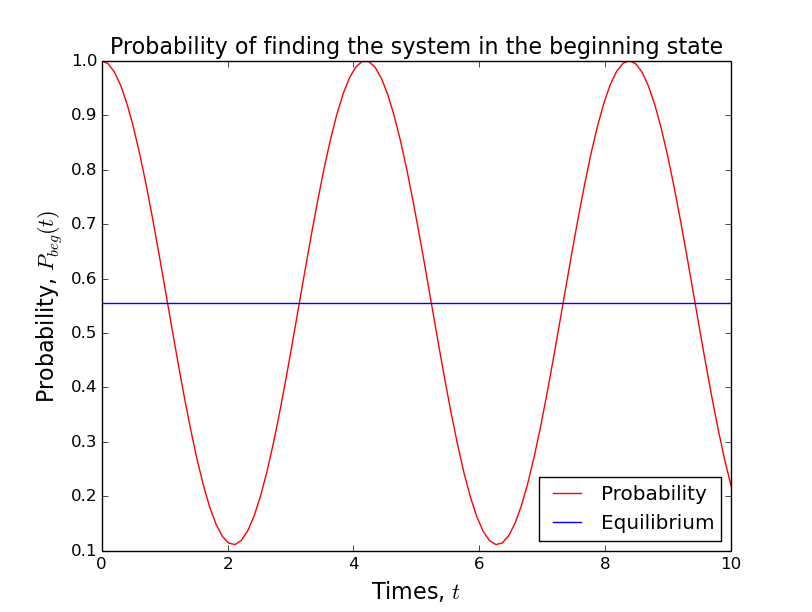
\includegraphics[width=150mm]{figure_1.png}
\caption{The probability of finding the system in the beginning state $\ket{\uparrow\downarrow\downarrow}$ after a time $t$. The constants $J$ and $\hbar$ are scaled to 1 \label{overflow}}
\end{figure}\par
\textit{Program 1 is found in the Code Attachment}

\newpage
\section*{Problem 2}
In this problem we are assuming that we know a Hamiltonian, although we do not know the ground state $\ket{E_0}$. We have a way to solve $\ket{\psi(s)}=e^{-\hat{H}s}\ket{\psi}$, $\forall s \in \!R$ with units energy inverse. How do we find an approximate expectation value $\mel{E_0}{\hat{O}}{E_0}$ for a hermitian operator $\hat{O}$?

\subsection*{2.1}
I will start expressing $\ket{\psi}$ as a sum over all the energy eigenstates of $\hat{H}$:
\begin{equation*}
\ket{\psi}=\sum_{i=0}^\infty c_i\ket{E_i}
\end{equation*}
Where $\ket{E_i}$ is eigenstate $i$ and $c_i$ is the corresponding coefficient. 
\begin{equation*}
\ket{\psi(s)}\equiv e^{-\hat{H}s}\ket{\psi}=e^{-\hat{H}s}\sum_{i=0}^\infty c_i\ket{E_i}=\sum_{i=0}^\infty c_ie^{-E_is}\ket{E_i}=c_0e^{-E_0s}\ket{E_0}+\sum_{i=1}^\infty c_ie^{-E_is}\ket{E_i}
\end{equation*}
Where $E_i$ is the eigenvalue (energy) of the eigenstate $\ket{E_i}$. $\ket{\psi(s)}$ is just a energy-evolution of $\ket{\psi}$, so we can think of the latter as $\ket{\psi(0)}$. We can change the operator in the exponent from $\hat{H}$ to $E_i$ due to the power series ($e^{\hat{A}}\ket{\psi}=e^{a}\ket{\psi}$ where $\ket{\psi}$ is an eigenstate of $\hat{A}$ and $a$ is the corresponding eigenvalue). Nevermind, we are interested in the ground state $\ket{E_0}$, which is given by
\begin{equation*}
\ket{E_0}=\frac{\ket{\psi(s)}-\sum_{i=1}^\infty c_ie^{-E_is}\ket{E_i}}{c_0e^{-E_0s}}
\end{equation*}
We can then express $\mel{E_0}{\hat{O}}{E_0}$ as
\begin{equation*}
\mel{E_0}{\hat{O}}{E_0}=\frac{\mel{\psi(s)}{\hat{O}}{\psi(s)}-\sum_{i=1}^\infty |c_i|^2e^{-2E_is}\mel{E_i}{\hat{O}}{E_i}}{|c_0|^2e^{-2E_0s}}
\end{equation*}
\begin{equation}
\mel{E_0}{\hat{O}}{E_0}=\frac{\mel{\psi(s)}{\hat{O}}{\psi(s)}}{\braket{\psi(s)}{\psi(s)}}-\sum_{i=1}^\infty \Big|\frac{c_i}{c_0}\Big|^2e^{-2(E_i-E_0)s}\mel{E_i}{\hat{O}}{E_i}
\label{eq:E0OE0}
\end{equation}
The ground state has always lowest eigenvalue, and we have $E_0<E_1<E_2...$ The exponent will therefore always be negative, so for large $s$'s the last term will be very small. We can make a approximation for large $s$'s ($s>>1$):
\begin{equation}
\mel{E_0}{\hat{O}}{E_0}\approx\frac{\mel{\psi(s)}{\hat{O}}{\psi(s)}}{\braket{\psi(s)}{\psi(s)}}
\label{eq:E0OE0approx}
\end{equation}
We can say that $\ket{E_0}$ is the dominating eigenstate for large $s$-values. But what about for small values if $s$? Then the eigenstate with largest eigenvalue will be dominating, and we can actually not express $\mel{E_0}{\hat{O}}{E_0}$ in a simpler way than in Equation (\ref{eq:E0OE0}).\par 
In general, the error decreases when we are increasing $s$. If we assume that the differences between the eigenvalues are constant $\Delta E$ (not a good assumption for natural processes, but in many cases good enough), we will better see how the error is varying for different values of $\Delta E\cdot s$. The $s$-dependent part of the sum is
\begin{equation}
\sum_{i=1}^\infty e^{-2(E_i-E_0)s}=\sum_{i=1}^\infty e^{-2i\Delta E\cdot s}
\label{eq:Error}
\end{equation}
When I plot this with $\Delta E\cdot s\in[10^{-8},4]$, we obtain the plot in \textit{Figure 2}.
\begin{figure}[!htbp]
\centering
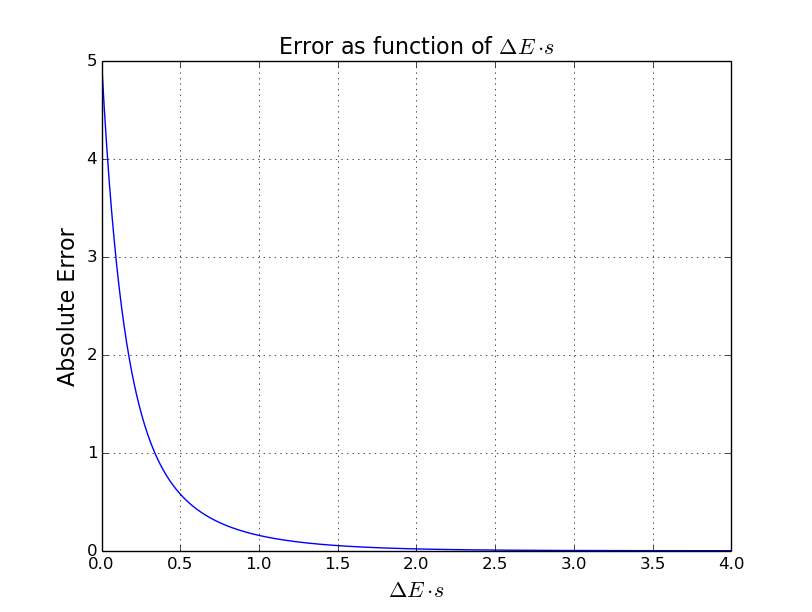
\includegraphics[width=150mm]{figure_2.png}
\caption{The absolute error plotted as function of $\Delta E\cdot s\in [1e-8,4]$ \label{overflow}}
\end{figure}\par
From \textit{Figure 2} we can see that the error is decreasing fast, and when $\Delta E\cdot s\approx 4$, the error approaches zero. This means the large $s$ approximation in Equation (\ref{eq:E0OE0approx}) is good when $\Delta E\cdot s > 4$. Above I have assumed that the eigenstates $\ket{\psi}$ are orthogonal, otherwise the inner product $\braket{\psi(s)}{\psi(s)}$ is zero, and Equation (\ref{eq:E0OE0}) and (\ref{eq:E0OE0approx}) go to infinity (cannot be real). 
\par\textit{Program 2 is found in the Code Attachment}

\newpage
\section*{Code Attachment}
\subsection*{Program 1}
I decided to use Python for making the plot from exercise 1.8. 
\lstinputlisting[language=Python]{Home_Exam_1.8.py}
First I define the constants $J$ and $\hbar$, which are scaled to be equal to 1 (the frequency of the probability change depends on $J$ and $\hbar$, but since we not have defined the unit of $t$, all choices of $J$ and $\hbar$ are valid). Furthermore I made a function prob which takes a time as argument and returns the corresponding probability. Then the probability is calculated for 10 time units, and plotted as function of this time.
\newpage
\subsection*{Program 2}
This is the script used to make the plot in exercise 2.1
\lstinputlisting[language=Python]{Home_Exam_2.1.py}
The program consists of a function which takes the number of terms and a value $\Delta E\cdot s$ as argument, and returns the absolute error calculated with the formula in Equation (\ref{eq:Error}). Then the error is plotted as function of 1000 points in range $\Delta E\cdot s\in [1e-8,4]$. 
\end{document}